%
%  hume.three
%
%  Created by Mark Eli Kalderon on 2007-08-03.
%  Copyright (c) 2007 Mark Eli Kalderon. All rights reserved.
%
%  Beamer

% Definitions and macros
\newcommand{\change}{\textcolor{blue}{\textbf{CHANGE SLIDE}}}
\newcommand\myauthor{Mark Eli Kalderon} 
\newcommand\mytitle{Introduction to Moral Philosophy}
\newcommand\mysubtitle{Hume}
\newcommand\myinstitution{University College London}
\newcommand\myurl{http://markelikalderon.com/teaching/}

% Packages specific to lecture notes
\mode<article>{
    \usepackage{palatino}
}

% Packages specific to beamer presentation
\mode<presentation>{
    \usetheme{Darmstadt}
    \setbeamercovered{transparent}
    \pgfdeclareimage[height=0.5cm]{university-logo}{../../../graphics/logo_sml_blk}
    \logo{\pgfuseimage{university-logo}}
}

% Packages common to lecture notes and beamer presentation
\usepackage{pgf}
\usepackage{tikz}
\usepackage{hyperref}

\setjobnamebeamerversion{hume.three.beamer}

\title{\mytitle}
\subtitle{\mysubtitle}

\author{\myauthor\\
\url{\myurl}}
\institute{\myinstitution}

% \date[Short Occasion] % (optional)
% {Date / Occasion}

\begin{document}

\frame{\maketitle}

\section{Review}\label{sec:review} % (fold)

\change\ So far we have seen a number of principles of Hume's new science of human nature. We have discussed the first principle of that science, `` that all our simple ideas in their first appearance are deriv’d from simple impressions, which are correspondent to them, and which they exactly represent''. Moreover, we have seen that ideas in the mind are not constant, but despite this inconstancy, their change is governed by a fixed principle, the association of ideas---that ideas that are related by the natural relations of resemblance, contiguity, and causation are related by a force akin to gravity or magnetism. So, for example, an idea will tend to occasion another idea that resembles it. Last time, we discussed two more principles of Hume's philosophical psychology, the \emph{association of impressions} and \emph{sympathy}. The association of impressions was deployed in Hume's account of the passion of pride. Pride is the result of the double association of ideas and impressions. Whereas ideas are associated by the relations of resemblance, contiguity, and causation, impressions are associated solely by resemblance. Suppose I am a proud of my beautiful house. My pleasure in the house's beauty resembles the pleasure of pride. Given the association of impressions, it occassions that passion. My idea of my beautiful house, being \emph{mine} and given the association of ideas, tends to occasion my idea of myself, the object of pride. Sympathy was introduced to handle the secondary causes of pride such as the esteem of another. In such cases, the pleasure of another tends to occastion the pleasure of pride in myself. The principle of the association of impressions cannot explain this since it is an \emph{intra}subjective principle governing the impressions that occur within the psychology of a \emph{single} individual. What's needed to account for the secondary causes of pride is an \emph{inter}subjective principle---a principle that coordinates the impressions within the psychologies of distinct individuals. Sympathy, as Hume inderstands it, is such a principle. As Hume understands it, sympathy is thus not a sentiment---what we call sympathy Hume would denominate as pity or compassion. Sympathy, rather, is a principle that coordinates the passions of distinct individuals. It is best understood not as a principle of emotional contagion since it can give rise to distinct if complementary passions---thus esteem gives rise to pride. So suppose my friend has received good news and this has made him happy. This passion, happiness, affects his appearance and behavior: He has a cheerful countenance, a bright smile, and a lively step. When I perceive his appearance and behavior, I take these as a sign of his happiness since I know from experience that such appearance and behavior is typically caused by that passion. Now my friend is related to me by resemblance and contiguity. My friend resembles me and not merely in the general manner in which all humans resemble one another. More than this, we share certain interests and concerns together. Moreover, he is contiguous with me---he has just greeted me to convey his good news. I have formed an idea of my friend's happiness. Since he is \emph{my} friend, related to me by resemblance and contiguity, my lively conception of myself lends its force and vivacity to my idea of my friend's happiness and converts this idea into the corresponding impression. I come to feel happy myself and so share in my friend's happiness. In this way, the relations of resemblance, contiguity, and causation transforms an idea of another's passion into a passion. \change

% \textbf{See Figure~\ref{fig:slide0}.}
% 
% \begin{figure}[ht]
%     \begin{center}
%         \includeslide[height=5cm]{slide0<1>}
%     \end{center}
%     \caption{Main Points from Last Time}
%     \label{fig:slide0}
% \end{figure}

\begin{frame}<presentation>[label=slide0]
    \frametitle{Main Points from Last Time}
        \begin{itemize}
        \item<1-> The Association of Impressions
        \item<2-> Sympathy
        \end{itemize}
\end{frame}

% section review (end)

\section{The Slave of the Passions}\label{sec:the_slave_of_the_passions} % (fold)

There is a familiar image, with a long tradition among philosophers and the vulgar alike, of the combat of reason and the passions. Among philosophers, the image dates back at least to Plato, and it played a dominant role in Stoic thought. The image is familiar as well in Hume's own time. Thus Pascal (pictured here) wrote of ``the internal war of reason and the passions'' (\emph{Pens\'{e}es}). Not only does the image of reason and passion's combat play an important role in philosophical reflection on the determinants of the will and human action, but it plays a role as well in the thought of the vulgar. We are inclined to speak of a person who, in the throws of violent emotion, acts contrary to his interests as being ``out of his senses''---the suggestion being that the operation of reason (involving, in this instance, the abilities to recognize what is in one's best interest and to take relevant steps to promote, or at least not frustrate, that interest) has been disordered by the turbulence of felt emotion.

The image of reason and passion's combat encourages a number of closely related claims:

\begin{itemize}
    \item Reason and the passions can both determine the will.
    \item The passions can oppose reason's determination of the will, and reason can oppose the passions' determination of the will.
    \item Reason \emph{ought} to determine the will.
\end{itemize}

A person is only virtuous to the extent that his will is determined by reason.
Suppose that reason ought to determine the will and that a person is only virtuous to the extent that his will is determined by reason. Then, if the will is determined by passions that oppose the operation of reason, one acts not only unreasonably but viciously as well. This led many thinkers to lament reason's enslavement to the passions. \change

% \textbf{See Figure~\ref{fig:slide1}}
% 
% \begin{figure}[ht]
%     \begin{center}
%         \includeslide[height=5cm]{slide1<1>}
%     \end{center}
%     \caption{The Combat of Reason and the Passions}
%     \label{fig:slide1}
% \end{figure}


\frame<presentation>[label=slide1]{
    \frametitle{The Comabt of Reason and the Passions}
        \begin{columns}
            \begin{column}{3cm}
                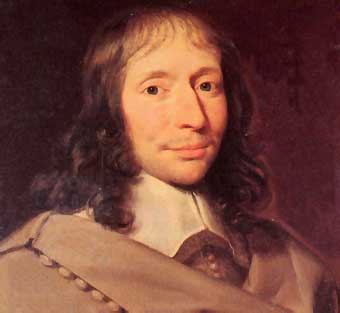
\includegraphics[width=3cm]{../../../graphics/pascal.jpg}
            \end{column}
            \begin{column}{6cm}
                 \begin{itemize}
                        \item Reason and the passions can both determine the will
                        \item The passions can oppose reason's determination of the will, and reason can oppose the passions' determination of the will
                        \item Reason \alert{ought} to determine the will
                    \end{itemize}
            \end{column}
       \end{columns}
}

Hume opposes this tradition, maintaining instead that (\emph{Treatise}, 2.3.3.2):

\begin{itemize}
    \item Reason \emph{alone} can never determine the will.
    \item Reason \emph{alone} can never oppose the passions' determination of the will.
\end{itemize}

Instead, reason has a more limited role to play. \change

% \textbf{See Figure~\ref{fig:slide2}}
% 
% \begin{figure}[ht]
%     \begin{center}
%         \includeslide[height=5cm]{slide2<1>}
%     \end{center}
%     \caption{Hume's Two Main Claims}
%     \label{fig:slide2}
% \end{figure}

\frame<presentation>[label=slide2]{
    \frametitle{Hume's Two Main Claims}
        \begin{columns}
            \begin{column}{3cm}
                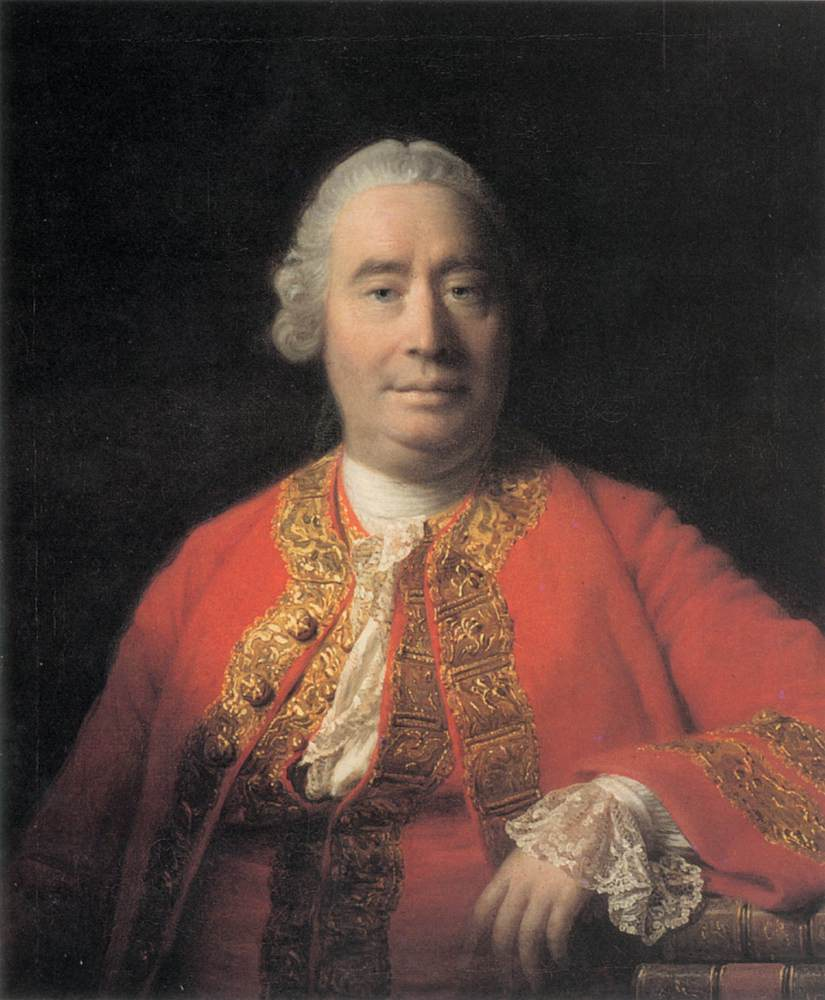
\includegraphics[width=3cm]{../../../graphics/hume.jpg}
            \end{column}
            \begin{column}{7cm}
                \begin{itemize}
                    \item Reason \alert{alone} can never determine the will
                    \item Reason \alert{alone} can never oppose the passions' determination of the will
                \end{itemize}
            \end{column}
        \end{columns}
}

The two functions of reason that Hume officially recognizes are as follows (\emph{Treatise}, 2.3.3.3):

\begin{itemize}
    \item Reason may \emph{demonstrate} certain truths based on the relations among our ideas (such as the truths of logic and mathematics).
    \item Reason may \emph{infer}, or render probable, on the basis of experience, that the relations of cause and effect obtain between objects and events.
\end{itemize}

Hume argues that neither operation suffices to determine the will and motivate human action.

Of course demonstrative truths can have a practical application. Hume observes that mathematics is useful to mechanics (understood, here, as engineering). So understood, mechanics is ``the art of regulating the motions of bodies \emph{to some design'd end or purpose}'' (\emph{Treatise}, 2.3.3.2). Mathematics is useful to mechanics since by means of it we can determine the proportion of causal influence of one body over another. However, the effectiveness of demonstrative reasoning, its influence on the will, \emph{presupposes} some end or purpose. Demonstrative reasoning may influence our actions---when, say, designing and building a bridge, but it does so only by directing our judgment concerning the propostion of causal influence. If a person did not have as an end the construction of a bridge, such causal judgments would have no influence on the will.

Similarly, causal truths can have a practical application. However, the effectiveness of causal reasoning, its influence on the will, \emph{presupposes} some end or purpose:

\begin{quote}
    It can never in the least concern us to know, that such objects are causes, and such others effects, if both the causes and effects be indifferent to us. Where the objects themselves do not affect us, their connexion can never give them any influence; and 'tis plain, that as reason is nothing but the discovery of this connexion, it cannot be by its means that the objects are able to affect us. (\emph{Treatise}, 2.3.3.3)
\end{quote}

Since reason is limited to demonstrating truths about the relations of ideas and inferring truths about cause and effect, and these alone cannot determine the will, Hume concludes that reason alone can never determine the will.

Since reason alone can never determine the will, neither can it oppose the passions' determination of the will. The passions' determination of the will could only be opposed by a contrary determination, but, as Hume has shown, reason alone can never determine the will:

\begin{quote}
    We speak not strictly and philosophically when we talk of the combat of passion and of reason. Reason is, and ought only to be the slave of the passions, and can never pretend to any other office than to serve and obey them. (\emph{Treatise}, 2.3.3.4)
\end{quote}

Hume is being deliberatively provocative here. To those who would lament reason's enslavement to the passions, Hume retorts that not only is reason the slave of the passions, but it \emph{ought only to be}. Notice that, in inverting the Stoic lament, Hume has also shifted the operative model of slavery. When, for example, Spinoza complains of our ``bondage'' to human passions, he has in mind the Egyptian enslavement of the Hebrews. When, however, Hume claims that reason is and ought only to be the slave of the passions, he has in mind the Roman enslavement of educated Greeks. Just as the influence of the Greek slaves over the Romans was limited to educating them, reason's influence over the will is limited to ``educating'' the passions as to the presence of their objects and the causal means to their obtainment. \change

% \textbf{See Figure~\ref{fig:slide3}}
% 
% \begin{figure}[ht]
%     \begin{center}
%         \includeslide[height=5cm]{slide3<1>}
%     \end{center}
%     \caption{Reason's Impotence}
%     \label{fig:slide3}
% \end{figure}

\frame<presentation>[label=slide3]{
    \frametitle{Reason's Impotence}
        \begin{columns}
            \begin{column}{3cm}
                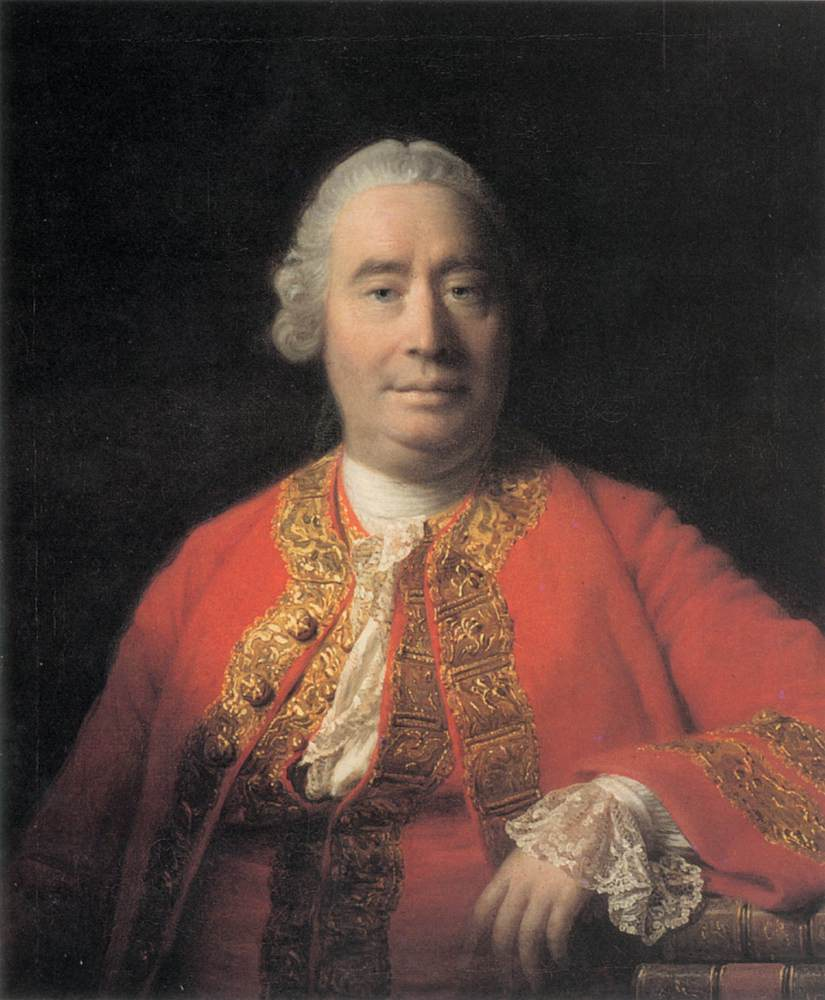
\includegraphics[width=3cm]{../../../graphics/hume.jpg}
            \end{column}
            \begin{column}{7cm}
                \alert{P1} Reason's operation is limited to:
                    \begin{itemize}
                        \item \small{Demonstrating truths on the basis of the relations among ideas}
                        \item \small{Inferring the relations of cause and effect on the basis of experience}
                    \end{itemize}
                \alert{P2} These cannot determine the will alone\\
                \alert{C} Reason cannot determine the will alone
            \end{column}
        \end{columns}
}

Two questions may be raised about Hume's case:

\begin{itemize}
    \item How can Hume validly conclude that reason \emph{ought only to be} the slave of the passions?
    \item Even if Hume's argument is valid, how convincing is it to someone who has a different conception of reason?
\end{itemize}

First, a question may be raised about the validity of Hume's argument. How is Hume entitled to the claim that reason \emph{ought} only to be the slave of the passions? From his premises, it may follow that reason is the slave of the passions---that reason can never determine the will nor oppose the passions' determination of the will. But that reason \emph{ought} only to be the slave of the passions is a further claim. I speculate that Hume is looking forward and backward here.

That reason to be the slave of the passions is the result of the self-vindicatory character of Hume's sentimentalist explanation of morals. Recall that Hume wants to describe and explain the moral judgments we make, rather than prescribe certain moral judgments and justify them. However, Hume believes that once we recognize how the moral judgments that we make are properly explained in terms of internal sentiment, we will naturally approve of them and the mechanisms that give rise to them. As a corollary, once we recognize reason's limited role in moral judgment we will naturally approve of reason's limited role. It is this sense of approbation that is the basis of the claim that reason ought to be the slave of the passions. So Hume is look forward to the conclusion of Book III where he discusses the self-vindicatory character of his sentimentalist explanation of morals.

That reason \emph{ought} only to be the slave of the passions is the result of Hume's skepticism. Recall that Book I concludes on a note of a despair. What Hume despairs of is the possibility of reasonable metaphysical speculation about the supersensible nature of things---for example, about the nature of the necessary connection between cause and effect. Given the temptation to engage in unreasonable metaphysical speculation, it is only proper that reason be passion's slave. For reason to pretend to any other office risks the kind of error that it is prone to when it engages in metaphysical speculation. So Hume is looking backward to the conclusion of Book I where he despairs of reason's limits.

Second, a question may be raised about the persuasiveness of Hume's argument. Even if valid, this line of argument may fail to convince, as Hume himself recognizes. The problem is that Hume's conclusion follows from his restricted conception of reason. One might concede that if reason is limited to demonstrating truths about the relations of ideas or inferring causal truths, then reason alone can never determine the will and hence never oppose the passions' determination of the will, and yet deny that reason's function is so limited. Reason, \emph{as Hume understands it} may never determine the will, but that is not yet to show that reason \emph{properly understood} never determines the will. \change

% \textbf{See Figure~\ref{fig:slide4}}
% 
% \begin{figure}[ht]
%     \begin{center}
%         \includeslide[height=5cm]{slide4<1>}
%     \end{center}
%     \caption{Two Questions}
%     \label{fig:slide4}
% \end{figure}

\frame<presentation>[label=slide4]{
    \frametitle{Two Questions}
        \begin{columns}
            \begin{column}{3cm}
                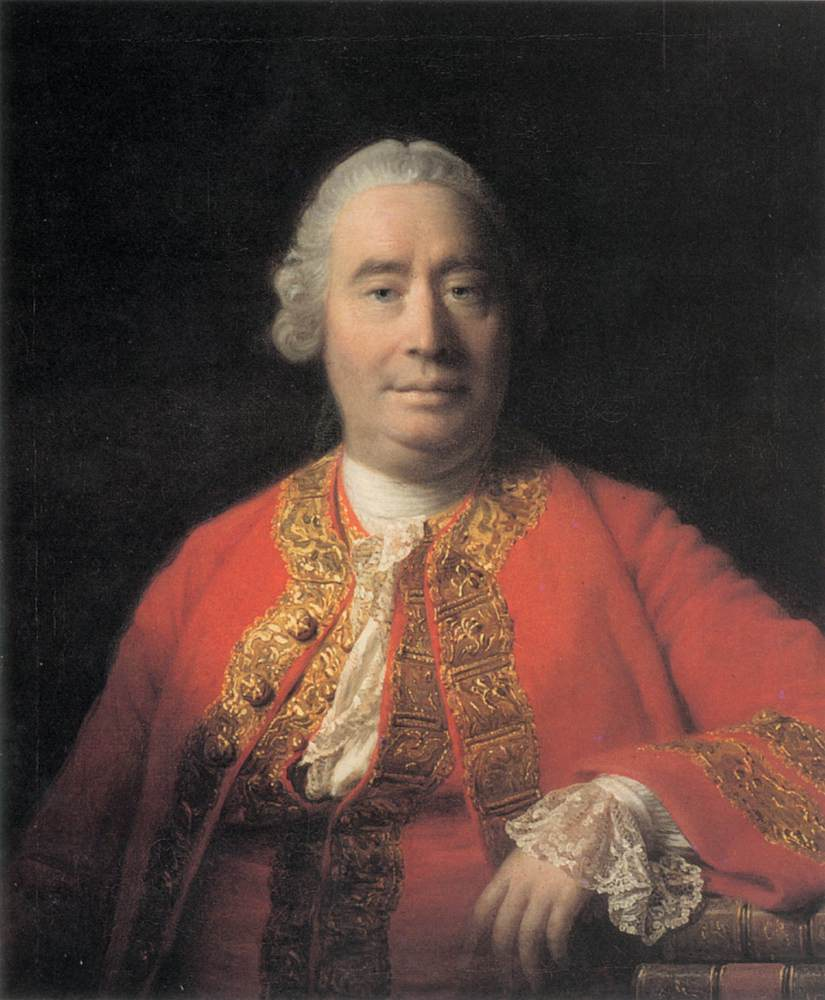
\includegraphics[width=3cm]{../../../graphics/hume.jpg}
            \end{column}
            \begin{column}{7cm}
                \begin{itemize}
                    \item How can Hume validly conclude that reason \alert{ought only to be} the slave of the passions?
                    \item Even if Hume's argument is valid, how convincing is it to someone who has a different conception of reason?
                \end{itemize}
            \end{column}
        \end{columns}
}

Hume recognizes this latter difficulty and provides an independent argument that the passions cannot be opposed by reason. Recall that passions are occurrent psychological episodes. They are simple impressions of reflection that arise under certain conditions and that prompt us to occasion further ideas and impressions and to act in certain ways. The passions are ``original existences'', and so cannot represent anything. According to Hume, for a thing to have a representative quality it must be the ``copy of another existence'', but the passions, being original existences are the copy of no other thing. Since the passions do not represent anything, they cannot contradict a truth discovered by reason.

Passions may not be opposed to reason by contradicting a truth discovered by reason, but perhaps the passions may be opposed to reason by certain judgments accompanying them contradicting a truth discovered by reason. Hume concedes that the passions may be contrary to reason, or unreasonable, in one of two ways:

\begin{itemize}
    \item When it is based on a false belief (e.g., when we are afraid of something because we falsely believe that it is dangerous).
    \item When a choice of a means to the passion's end is unreasonable, when the means do not have the expected effect.
\end{itemize}

But so conceding concedes little: ``Where a passion is neither founded on false suppositions, nor chooses means insufficient for the end, the understanding can neither justify nor condemn it.'' (\emph{Treatise}, 2.3.3.6)

Hume underscores this point in an extraordinary passage:

\begin{quote}
    \'Tis not contrary to reason to prefer the destruction of the whole world to the scratching of my finger. \'Tis not contrary to reason for me to choose my total ruin, to prevent the least uneasiness of an Indian or person wholly unknown to me. \'Tis as little contrary to reason to prefer even my own acknowledg'd lesser good to my greater, and have a more ardent affection for the former than the latter. A trivial good may, from certain circumstances, produce a desire superior to what arises from the greatest and most valuable enjoyment; nor is there anything more extraordinary in this, than in mechanics to see one pound weight raise up a hundred by the advantage of its situation. (\emph{Treatise}, 2.3.3.6)
\end{quote}

Again, Hume is being deliberatively provocative. It may no be contrary to reason to prefer the destruction of the whole world to the scratching of my finger in the strict and philosophical sense of reason, but there is another sense of reason familiar to the vulgar in which it would be utterly mad, insane, to prefer this. Hume invites this response, for, as we will see, it sets up his diagnosis of the mistake we make in speaking of the combat of reason and the passions. \change

% \textbf{See Figure~\ref{fig:slide5}}
% 
% \begin{figure}[ht]
%     \begin{center}
%         \includeslide[height=5cm]{slide5<1>}
%     \end{center}
%     \caption{The Master Argument}
%     \label{fig:slide5}
% \end{figure}

\frame<presentation>[label=slide5]{
    \frametitle{The Master Argument}
        \begin{columns}
            \begin{column}{3cm}
                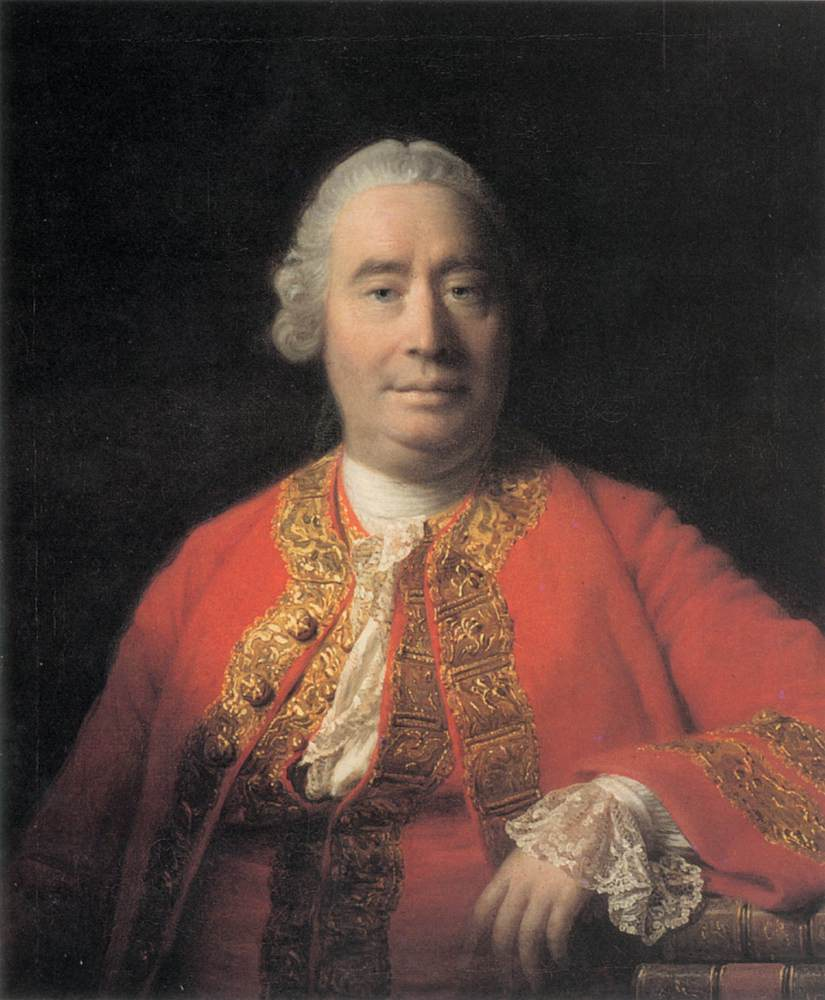
\includegraphics[width=3cm]{../../../graphics/hume.jpg}
            \end{column}
            \begin{column}{7cm}
                \alert{P1} For something to have a representative quality it must be \alert{the copy of another existence}\\
                \alert{P2} Passions are \alert{original existences} and so the copy of no other thing\\
                \alert{C} Since the passions do not represent anything, they cannot be contrary to reason
            \end{column}
        \end{columns}
}

Before we discuss Hume's diagnosis, let's first observe that, for Hume, preferences and value are independent of one another. A person may prefer what he judges to be a lesser good to a greater good (or a lesser pleasure to a greater pleasure---Hume regards pleasure and goodness as more or less equivalent). Hume's metaphysics of mind commits him to this psychological claim. A person's preferences are determined by his passions, and as these are original existences, they are independent of expectations of pleasure. So it is possible for a person to prefer an object that he expects to produce less pleasure than any other alternative. In this passage, all of Hume's examples take this form. When a person prefers the destruction of the whole world to the scratching of his finger, he prefers something incompatible with his good. The same is true of preferring total ruin to prevent the least uneasiness in a person wholly unknown to oneself. Indeed the vulgar response that such preferences are utterly mad, insane, are due to their being contrary to the good and the sheer magnitude of this contrast.

When philosophers and the vulgar claim that reason can determine the will and oppose the passions' determination of the will, they mistake the operation of certain calm passions for the operation of reason. Recall that the passions are either calm or violent. Calm passions ``though they be real passions produce little emotion in the mind and are more known by their effects than by the immediate feeling of sensation'' (\emph{Treatise}, 2.3.3.8). In this way, they differ from violent passions which can be known by immediate feeling or sensation. Since reason itself exerts little sensible emotion, it is natural to mistake the operation of the calm passions, for the operation of reason.

What the vulgar call ``passions'' are really violent emotions that arise from any good or evil that excites that appetite. What the vulgar call ``reason'' are really emotions that operate more calmly and occasion no disorder. The calm passions include, among others, the general appetite to good and aversion to evil. Consider now the case of someone preferring the destruction of the whole world to the scratching of his finger. In this case, a strong violent emotion has overcome the weak general appetite for the good that operates more calmly and occasions no such disorder. This preference is not contrary to reason in the strict and philosophical sense. Rather, this preference occasions the distinctive pain of disapprobation from a more general point of view in characters where the calm passions operate more strongly. When the vulgar describe the preference for the destruction of the whole world as unreasonable, mad, insane, they are really giving confused expression to this sense of disapprobation. \change

% \textbf{See Figure~\ref{fig:slide6}}
% 
% \begin{figure}[ht]
%     \begin{center}
%         \includeslide[height=5cm]{slide6<1>}
%     \end{center}
%     \caption{Calm and Violent Passions}
%     \label{fig:slide6}
% \end{figure}

\frame<presentation>[label=slide6]{
    \frametitle{Calm and Violent Passions}
        \begin{columns}
            \begin{column}{3cm}
                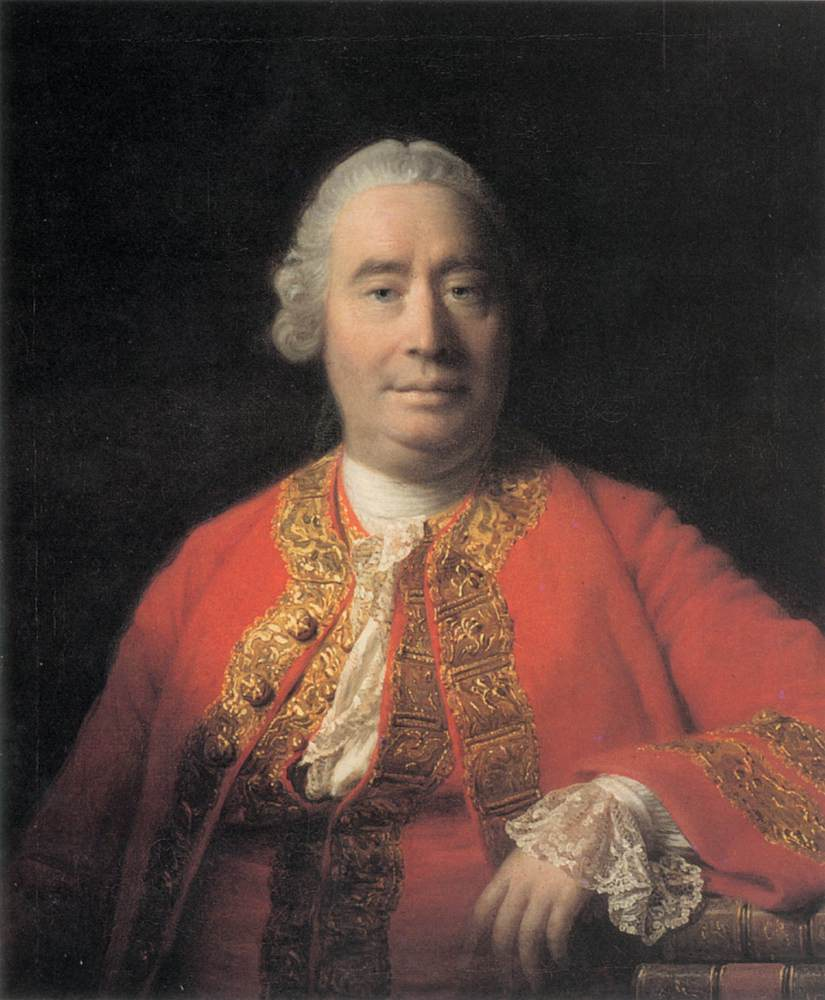
\includegraphics[width=3cm]{../../../graphics/hume.jpg}
            \end{column}
            \begin{column}{7cm}
                \begin{itemize}
                    \item In the \alert{strict and philosophical sense} there could be no combat between reason and the passions
                    \item The vulgar mistake \alert{the operation of the calm passions} for \alert{the operation of reason}
                    \item At best, \alert{passion in the vulgar} sense is a violent passion, and \alert{reason in the vulgar sense} is a calm passion
                \end{itemize}
            \end{column}
        \end{columns}
}

% section the_slave_of_the_passions (end)

\section{Reason Not the Source of Moral Distinctions}\label{sec:reason_not_the_source_of_moral_distinctions} % (fold)

Recall the elements of Hume's metaphysics of mind. Whatever is present to the mind is a perception, and all the actions of the mind count as perceptions. Perceptions are either impressions or ideas depending on their relative force or vivacity. With these distinctions in place, Hume raises the question:

\begin{quote}
    Whether 'tis by means of our ideas or impressions we distinguish betwixt vice and virtue, and pronounce an action blameable or praise-worthy? (\emph{Treatise}, 3.1.1.3)
\end{quote}

Hume regards this as a more precise form of the question that divided \emph{moral rationalists} (such as Malebranche, Clarke, and Cudworth) and \emph{moral sentimentalists} (such as Shaftesbury and Hutcheson):

\begin{quote}
    Whether moral distinctions are determined by reason or internal sentiment?
\end{quote}

According to moral rationalists, virtue is nothing but conformity to reason. As Hume interprets this doctrine, the rationalists are committed to the claim that the distinction between vice and virtue is determined by the relations among ideas and so demonstrable by reason. If Hume can show that the distinction between vice and virtue is not determined by means of our ideas, this will be sufficient grounds for rejecting the central claims of the moral rationalists, and so settle this debate in favor of moral sentimentalism.

One question to bear in mind: Is Hume's more precise question an acceptable substitute for the question that drives the traditional pre-Humean debate between rationalists and sentimentalists? Does settling whether moral distinctions are drawn by means of ideas or impressions really settle the question of whether moral distinctions are determined by reason or internal sentiment? \change

% \textbf{See Figure~\ref{fig:slide7}.}
% 
% \begin{figure}[ht]
%     \begin{center}
%         \includeslide[height=5cm]{slide7<1>}
%     \end{center}
%     \caption{The Question of 3.1.1--2}
%     \label{fig:slide7}
% \end{figure}

\frame<presentation>[label=slide7]{
    \frametitle{The Question of 3.1.1--2}
        \begin{columns}
            \begin{column}{3cm}
                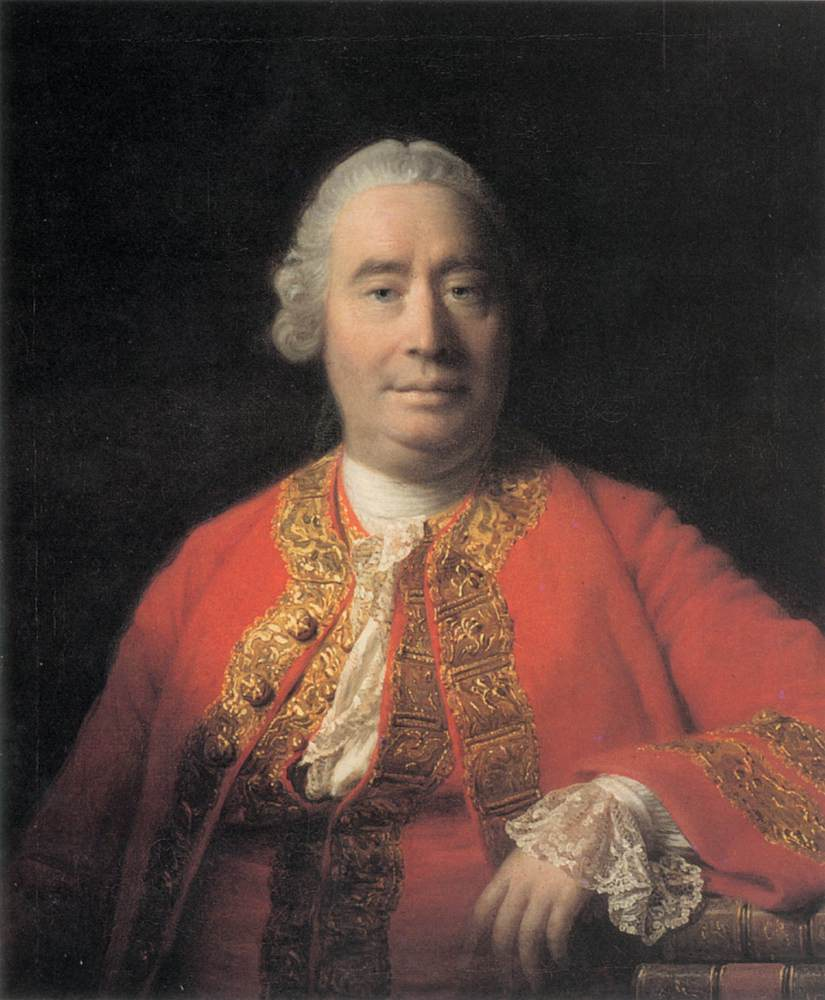
\includegraphics[width=3cm]{../../../graphics/hume.jpg}
            \end{column}
            \begin{column}{7cm}
                \begin{quote}
                    Whether 'tis by means of our ideas or impressions we distinguish betwixt vice and virtue, and pronounce an action blameable or praise-worthy?
                \end{quote}
                Hume regards this as a more precise version of the question:
                \begin{quote}
                    Whether moral distinctions are determined by reason or internal sentiment?
                \end{quote}
            \end{column}
        \end{columns}
}

Hume begins by observing that morals has an influence on the will and human action:

\begin{quote}
    Philosophy is commonly divided into speculative and practical; and as morality is always comprehended under the latter division, 'tis suppos'd to influence our passions and actions, and to go beyond the calm and indolent judgements of the understanding. And this is confirm'd by commone experience, which informs us, that men are often govern'd by their duties, and are deter'd from some actions by the opinions of injustice, and impell'd to others by that of obligation.
\end{quote}

We have seen how in \emph{Treatise} 2.3.3 Hume argues for the claim that reason alone can never determine the will. In \emph{Treatise} 3.1.1, this important claim emerges as a central premise of Hume's main argument against moral rationalism:

\begin{quote}
    Since morals, therefore, have an influence on the actions and affections, it follows, that they cannot be deriv'd from reason; and that because reason alone, as we have already prov'd, can never have any such influence. Morals excite passions, and produce or prevent actions. Reason of itself is utterly impotent in this particular. The rules of morality, therefore, are not conclusions of our reason. (\emph{Treatise}, 3.1.1.6)
\end{quote}


More schematically, we can represent Hume's argument as follows:

\begin{enumerate}
    \item Reason alone cannot influence passions and actions.
    \item Moral distinctions can influence passions and actions.
    \item Therefore, moral distinctions are not discovered by reason.
\end{enumerate}

Hume observes that the argument is valid, and regards the second premise as evident from cautious observation of human action, and so concludes that the only way to resist this argument is to deny the first premise, that reason alone cannot influence the passions and actions. He repeats the main argument of \emph{Treatise} 2.3.3 (that passions are original existences, and so lack a representative quality, and so cannot be contrary to a truth discovered by reason), and supplements this with a battery of subsidiary arguments. \change

% \textbf{See Figure~\ref{fig:slide8}.}
% 
% \begin{figure}[ht]
%     \begin{center}
%         \includeslide[height=5cm]{slide8<1>}
%     \end{center}
%     \caption{Hume's First Argument}
%     \label{fig:slide8}
% \end{figure}

\frame<presentation>[label=slide8]{
    \frametitle{Hume's First Argument}
            \begin{columns}
                \begin{column}{3cm}
                    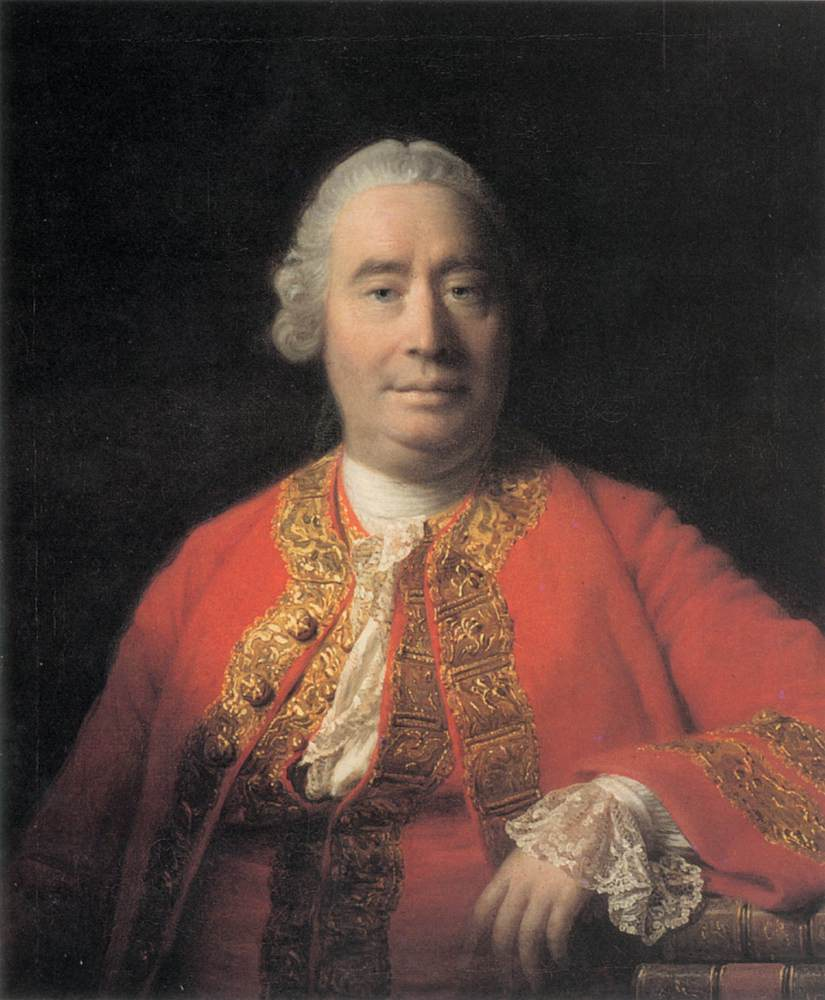
\includegraphics[width=3cm]{../../../graphics/hume.jpg}
                \end{column}
                \begin{column}{7cm}
                    \alert{P1} Reason alone cannot influence passions and actions\\
                    \alert{P2} Moral distinctions can influence passions and actions\\
                    \alert{C} Therefore, moral distinctions are not discovered by reason
                \end{column}
            \end{columns}
}

Hume's second argument against moral rationalism occurs in \emph{Treatise}, 3.1.1.18--25. Moral rationalists maintain that morality is susceptible to demonstration. According to Hume, demonstrable truths are determined by the relations among ideas. Specially, among the philosophical relations there are four that are capable of demonstration:

\begin{itemize}
	\item Resemblance
	\item Contrariety
	\item Degrees in quality
	\item Proportions in quantity and number
\end{itemize}

If moral distinctions really are demonstrable, then we must be able to discern them on the basis of one or more of these relations. Moral distinctions pertain exclusively to our actions, passions and volitions. However, the four demonstrable relations obtain not only among our actions, passions, and volitions, but among inanimate objects as well. So, the distinction between vice and virtue cannot be demonstrated on the basis of them.

The moral rationalist might concede that moral distinctions cannot be demonstrated on the basis of resemblance, contrariety, degrees in quality, or proportions of quantity and number. They might maintain, instead, that moral distinctions are demonstrable on the basis of some other relation. (Thus, one moral rationalist, Clarke, speaks of the relations of fittingness and unfittingness that virtuous and vicious actions bear to the circumstances in which they are performed.) If the moral rationalist is tempted to make this reply, Hume contends that he must explicitly specify the novel relations, and do so subject to two conditions:

\begin{itemize}
	\item First, the relations must obtain between perceptions in the mind and external objects.
	\item Second, the relations, being demonstrable, are knowable a priori and cause everyone that knows them to act virtuously to some degree.
\end{itemize}

However, Hume doubts that these two conditions can be met.

First, the relations must obtain between perceptions in the mind and external objects. The relations could not obtain between perceptions alone or external objects alone. If what made for vice are relations that obtain between perceptions, it would be possible to be guilty of some vice independently of our external circumstances, but that's implausible. If what made for vice are relations that obtain between external objects, then it would be possible for inanimate objects to be guilty of some vice, but that is implausible as well. So the relevant relations must obtain between perceptions in the mind and external objects. However, Hume contends that it is difficult to imagine a relation that obtains between perceptions and external objects that could not also obtain between perceptions alone, or external objects alone. So, it is implausible that the moral rationalist can successfully meet the first condition.

Second, the relations, being demonstrable, are knowable a priori and cause everyone that knows them to act virtuously to some degree:

\begin{quote}
	\ldots 'tis not only suppos'd, that these relations, being eternal and immutable, are the same, when consider'd by every rational creature, but their effects are also suppos'd to be necessarily the same; and 'tis concluded they have no less, or rather a greater, influence in directing the will on the deity, than in governing the rational and virtuous of our own species. (Treatise, 3.1.1.22)
\end{quote}


However, ``[t]hese two particulars are evidently distinct'':

\begin{quote}
	\'Tis one thing to know virtue, and another to conform the will to it. In order, therefore, to prove, that the measures of right and wrong are eternal laws, obligatory on every rational mind, 'tis not sufficient to show the relations upon which they are founded: We must also point out the connexion betwixt the relation and the will; and must prove that this connexion is so necessary, that in every well-dispos'd mind, it must take place and have its influence; tho' the difference betwixt these minds be in other respects immense and infinite. (Treatise,3.1.1.22)
\end{quote}

The problem is that there could be no proof of this necessary connection. The relations are demonstrable and so knowable independently of experience, but the causal effects of the relation could only be known on the basis of experience. According to Hume, then, the moral rationalists fail to successfully integrate their moral epistemology with an adequate explanation of moral motivation. So, it is implausible that the moral rationalist can successfully meet the second condition. (This is the source of John Mackie's notorious ``argument from queerness''.) \change

% section reason_not_the_source_of_moral_distinctions (end)

\section{Next Time}\label{sec:readings_for_next_time} % (fold)

% \textbf{See Figure~\ref{fig:slide13}.}
% 
% \begin{figure}[ht]
%     \begin{center}
%         \includeslide[height=5cm]{slide13<1>}
%     \end{center}
%     \caption{Readings for Next Time}
%     \label{fig:slide13}
% \end{figure}

\begin{frame}<presentation>[label=slide13]
    \frametitle{Readings for Next Time}
        Required:
        \begin{itemize}
            \item 3.2.1--3
        \end{itemize}
\end{frame}




% section readings_for_next_time (end)

\section{Next Time}\label{sec:next_time} % (fold)



% section next_time (end)

\end{document}
